\documentclass[oneside]{book}

\usepackage[utf8]{inputenc}
\usepackage{color}
\usepackage[english]{babel}
\usepackage[ruled,vlined,noend]{algorithm2e}
\usepackage{amsmath}
\usepackage[normalem]{ulem}
\newcommand{\stkout}[1]{\ifmmode\text{\sout{\ensuremath{#1}}}\else\sout{#1}\fi}
\usepackage[]{hyperref}

\usepackage[top=1in, bottom=1.25in, left=1.25in, right=1.25in]{geometry}

%%%%%%%%%%%%%%%CRISTINA%%%%%%%%%%%%%%%%%%%
\newcommand{\el}{$\mathcal{EL}$\xspace}
\newcommand{\elho}{$\mathcal{ELHO}^r_\bot$\xspace}
\newcommand{\shiq}{$\mathcal{SHIQ}$\xspace}
\newcommand{\hshiq}{Horn-\shiq\xspace}

\newcommand{\Onto}{\mathcal{O}}
\newcommand{\T}{\mathcal{T}}
\newcommand{\A}{\mathcal{A}}
\newcommand{\OKB}{\Onto=\langle\T,\A\rangle}

\newcommand{\dlisa}{\sqsubseteq}
\newcommand{\dland}{\sqcap}
\newcommand{\dlor}{\sqcup}
%%%%%%%%%%%%%%%CRISTINA%%%%%%%%%%%%%%%%%%%






\begin{document}

\title{\bf Enhancing the DLV system for\\large-scale ontology reasoning \\ \ \\
\Large \em Preliminary Report
\\ \ \\ }
\author{The authors go here}

%\date{December 2004}
\maketitle

\pagenumbering{Roman}

\chapter*{Summary}
%\addcontentsline{toc}{chapter}{Abstract}
The summary goes here...


\tableofcontents
\listoffigures
\listoftables


\chapter*{Introduction}
\addcontentsline{toc}{chapter}{\numberline{}Introduction}
\markright{Introduction}
\pagenumbering{arabic}

%\renewcommand{\abstractname}{Executive Summary}
% \begin{abstract}
% \addcontentsline{toc}{chapter}{Abstract}
% The abstract goes here...
% ...
% \end{abstract}

%%%%%%%%%%%%%%%%%%%%%%%%%%%%%%%%%%%%%%%%%%%%%%%%%%%%%%%%%%%%%%%%%%%%%%%%%%%%%%%%%%%%%%%%%%%%%%%%%%%%%%%%%%%%%%%%%%%%%%%%
%%%%%%%%%%%%%%%%%%%%%%%%%%%%%%%%%%%%%%%%%%%%%%%%%%%%%%%%%%%%%%%%%%%%%%%%%%%%%%%%%%%%%%%%%%%%%%%%%%%%%%%%%%%%%%%%%%%%%%%%
%%%%%%%%%%%%%%%%%%%%%%%%%%%%%%%%%%%%%%%%%%%%%%%%%%%%%%%%%%%%%%%%%%%%%%%%%%%%%%%%%%%%%%%%%%%%%%%%%%%%%%%%%%%%%%%%%%%%%%%%



\part*{Work Package 1:\\Data Loading Procedure Extensions}
\addcontentsline{toc}{part}{WP1: Data Loading Procedure Extensions}

\chapter{Scenario and problem description}

DLV natively supports the ASP formalism that requires data to be represented as a set of relational facts. One of the goals of this project is to extend the system in order to deal with OWL TBoxes in RDF/XML format, RDF ABoxes in Turtle format and Conjunctive Queries in SPARQL. In particular, a ``rewriting-based'' approach for handling OWL ontologies and SPARQL queries will be designed and developed within WP2; whereas, an extension of the system for loading Turtle ABoxes has been developed within WP1. 
BLA BLA BLA…

\section{Team}
WP1 has been fully developed by DLVSystem. In particular, what follows is the list of the involved researchers: Stefano Germano (PostDoc), Pierfrancesco Veltri (PostDoc), Jessica Zangari (PostDoc).



\section{The Turtle standard - Terse RDF Triple Language\texorpdfstring{\protect\footnote{From \url{https://www.w3.org/TR/turtle}}}{}}

We refer to RDF 1.1 Turtle as reported in its latest published version, available at \url{http://www.w3.org/TR/2014/REC-turtle-20140225/}.

The Resource Description Framework (RDF) is a general-purpose language for representing information in the Web.
We use a textual syntax for RDF called Turtle that allows an RDF graph to be completely written in a compact and natural text form, with abbreviations for common usage patterns and datatypes.

A Turtle document allows writing down an RDF graph in a compact textual form. An RDF graph is made up of triples consisting of a subject, predicate and object.\\
Comments may be given after a '\#' that is not part of another lexical token and continue to the end of the line.

The simplest triple statement is a sequence of (subject, predicate, object) terms, separated by whitespace and terminated by '.' after each triple.

Often the same subject will be referenced by a number of predicates. The predicateObjectList production matches a series of predicates and objects, separated by ';', following a subject. This expresses a series of RDF Triples with that subject and each predicate and object allocated to one triple. Thus, the ';' symbol is used to repeat the subject of triples that vary only in predicate and object RDF terms.
As with predicates often objects are repeated with the same subject and predicate. The objectList production matches a series of objects separated by ',' following a predicate. This expresses a series of RDF Triples with the corresponding subject and predicate and each object allocated to one triple. Thus, the ',' symbol is used to repeat the subject and predicate of triples that only differ in the object RDF term.

IRIs may be written as relative or absolute IRIs or prefixed names. Relative and absolute IRIs are enclosed in '<' and '>'.\\
Relative IRIs are resolved relative to the current base IRI. A new base IRI can be defined using the '@base' or 'BASE' directive.\\
The token 'a' in the predicate position of a Turtle triple represents the IRI\\
\verb|http://www.w3.org/1999/02/22-rdf-syntax-ns#type|.\\
A prefixed name is a prefix label and a local part, separated by a colon ":". A prefixed name is turned into an IRI by concatenating the IRI associated with the prefix and the local part. The '@prefix' or 'PREFIX' directive associates a prefix label with an IRI. Subsequent '@prefix' or 'PREFIX' directives may re-map the same prefix label.

Literals are used to identify values such as strings, numbers, dates.\\
Quoted Literals have a lexical form followed by a language tag, a datatype IRI, or neither.

\section{State of the art of Turtle parsing in C++}

\subsection{RDF Turtle management tools in C++}
There are C++ tools which provide parsing, serialising and management of RDF triples in the Turtle format.

The advantages of using an existing (and widely-used) tool are the stability, the correctness and the performance. The main disadvantage is the difficulty in customizing and adapting it to our needs (for example in terms of memory and time performance).

The most well-known (and widely-used) is the \href{http://librdf.org/raptor}{Raptor RDF Syntax Library}.\\
However, the latest version of this library is from 2014.\\
Moreover, their ``Turtle Parser'' is outdated; \href{https://www.w3.org/TR/turtle}{the latest version of the standard is from 2014} but they support an older one, as reported in their documentation:
\begin{quote}
\textit{A parser for the \href{http://www.w3.org/TR/2013/CR-turtle-20130219/}{Turtle Terse RDF Triple Language} W3C Candidate Recommendation, 19 February 2013 based on earlier work \href{http://www.dajobe.org/2004/01/turtle/}{Turtle Terse RDF Triple Language} (2004)}
\end{quote}

There are other libraries (for instance those on \href{https://sourceforge.net/directory/language:cpp/os:windows/?q=turtle}{SourceForge} or on \href{https://github.com/topics/turtle?l=c\%2B\%2B}{GitHub}), but none of these are stable enough for our purposes.

\textbf{Therefore, we decided to use a library and to perform the parsing manually.}\\
Although this requires a more extensive set of test and benchmarks in order to assess the correctness and the performance of the Turtle parser.

\subsection{Parsing libraries in C++}
There is no ``standard'' (or ``official'') way of performing parsing in C++.\\
However, in the latest 50 years many different alternatives have been proposed (see, for instance, \href{https://en.wikipedia.org/wiki/Comparison_of_parser_generators}{here}).
Starting from Lex and Yacc, nowadays replaced by \href{https://github.com/westes/flex}{Flex} and \href{https://www.gnu.org/software/bison}{Bison} (or \href{https://invisible-island.net/byacc}{Berkeley Yacc}, which claims to be ``\textit{the \href{https://web.archive.org/web/20130327184430/http://foldoc.org/byacc}{best yacc variant} available}''). They are the most popular and used by the C++ community. \href{http://dinosaur.compilertools.net}{These tools} are also well supported and used by several popular projects. However, everyone agrees that they are extremely difficult to develop and to debug.\\
Flex and Bison are also used in the current implementation of the I-DLV parser (for ASP programs).

Other popular C++ scanners and parsers generators are \href{http://re2c.org}{re2c}, \href{https://www.boost.org/doc/libs/1_68_0/libs/spirit}{Boost Spirit}, \href{http://www.antlr.org}{ANTLR}.\\
re2c seems to be (no actual reference) two or three times faster than flex, but it is less contributors and seems to be less used than flex.\\
Boost Spirit is believed (there are no actual tests) to be slower than Bison, but in the latest years it was hugely improved.\\
ANTLR has several advantages (for instance, plugins for the major programming IDEs and several standalone graphical IDEs that help the development of the grammar, or \href{https://github.com/antlr/grammars-v4/blob/master/turtle/TURTLE.g4}{an existing grammar for Turtle}), but it creates an LL parser (so it is easier to debug but slower) with a big memory footprint (users report this, there are no ``official'' comparisons).

Since the combination \emph{Flex+Bison} is already used in I-DLV (and therefore we do not have compliance or licensing issues) and since their performance are quite good and (seem to) fit our purpose, \textbf{we decided to use the \emph{Flex} and \emph{Bison} libraries to build the \emph{Turtle parser}}.



\section{Activity title}
TODO
\chapter{Results}
\chapter{Open research issues}
\chapter{Bibliography}
\chapter{Appendix}


%%%%%%%%%%%%%%%%%%%%%%%%%%%%%%%%%%%%%%%%%%%%%%%%%%%%%%%%%%%%%%%%%%%%%%%%%%%%%%%%%%%%%%%%%%%%%%%%%%%%%%%%%%%%%%%%%%%%%%%%
%%%%%%%%%%%%%%%%%%%%%%%%%%%%%%%%%%%%%%%%%%%%%%%%%%%%%%%%%%%%%%%%%%%%%%%%%%%%%%%%%%%%%%%%%%%%%%%%%%%%%%%%%%%%%%%%%%%%%%%%
%%%%%%%%%%%%%%%%%%%%%%%%%%%%%%%%%%%%%%%%%%%%%%%%%%%%%%%%%%%%%%%%%%%%%%%%%%%%%%%%%%%%%%%%%%%%%%%%%%%%%%%%%%%%%%%%%%%%%%%%

\setcounter{chapter}{0}

\part*{Work Package 2:\\Enhancing the Query Rewriting Techniques}
\addcontentsline{toc}{part}{WP2: Enhancing the Query Rewriting Techniques}

\chapter{Scenario and problem description}

We aim at extending DLV for answering Conjunctive Queries (CQs) over Horn-SHIQ ontologies by following a Datalog-rewriting approach. To this aim, nice algorithms have been introduced in the literature in the last few years. One of the goals of WP2 is to design and develop an optimized algorithm for (Datalog-)rewriting CQs over Horn-SHIQ ontologies, after studying state-of-the-art approaches proposed in the literature. Moreover, WP2 aims at improving the existing DLV rewriting technique called Magic Sets for dealing with Datalog-rewritings of OWL knowledge bases. 
BLA BLA BLA…

\section{Team}
WP2 has been jointly performed by DLVSystem, SRUK and DeMaCS@UNICAL. In particular, what follows is the list of the involved researchers: Mario Alviano (Professor), Cristina Civili (PostDoc), Marco Manna (Professor), Pierfrancesco Veltri (PostDoc).

\section{Horn-SHIQ Query Rewriting (Activity 2.1)}
In this section we show how to reduce query answering over \hshiq ontologies
to query answering over Datalog, independently from the ABox.
%
More formally, from a \hshiq TBox $\T$ and a conjunctive
query $q$, we construct a Datalog program $cr(\T)$ and a union of conjunctive queries $Q_{\T}$ such that, for each ABox $\A$, $\mathit{ans}(q,\A,\T) =  
\mathit{ans}(Q_{\T},\A \cup cr(\T))$. Note also that $cr(\T)$ is independent from $q$.


\subsection{Basics}

In \shiq, concepts have the form:

\[
\begin{array}{lllll}
A &  \top & \bot & \neg C & C \dland D \\
C \dlor D & \exists R.C & \forall R.C & \geq n S.C & \leq m S.C
\end{array}
\]

Roles have the form:

\[
\begin{array}{ll}
R &  R^-\\
\end{array}
\]

Axioms have the form:

\[
\begin{array}{ll}
\text{Role inclusion} & R_1 \dlisa R_2 \\
\text{Role transitivity} & Tra(R) \\
\text{Concept inclusion} & C_1 \dlisa C_2
\end{array}
\] 

The definition of a \hshiq ontology is based on the notion of polarity. A \shiq ontology  $\cal O$ is Horn if:


\begin{itemize}
	\item no concept of the form $C \dlor D$ or $\leq mR.C$ with $m > 1$ occurs positively in $\cal O$;
	\item no concept of the form $\neg C$, $\forall R.C$, $\geq n R.C$ with $n > 1$, or $\leq mR.C$ occurs negatively in $\cal O$.
	
\end{itemize}

\textbf{Polarities} \- Positive and negative polarities of occurrences of \shiq concepts
in concepts and axioms are defined as follows:

\begin{itemize}
	\item $C$ occurs positively in $C$;
	\item $C$ occurs positively (resp., negatively) in concepts of the form $\neg C_-$ if $C$ occurs negatively (resp., positively) in $C_-$;
	\item $C$ occurs positively (resp., negatively) in concepts of the form $C_+ \dland D_+$, $C_+ \dlor D_+$ if $C$ occurs positively (resp., negatively) in concepts of the form $C_+$ or in $D_+$;
	\item $C$ occurs positively (resp., negatively) in concepts of the form $\exists R.C_+$, $\forall R.C_+$, $\geq nS.C_+$, if $C$ occurs positively (resp., negatively) in $C_+$;
	\item $C$ occurs positively (resp., negatively) in $\leq mS.C_-$ if $C$ occurs  negatively (resp., positively) in $C_-$;
	\item $C$ occurs positively (resp., negatively) in axioms of the form  $C_- \dlisa D_+$ if $C$ occurs negatively (resp., positively) in $C_-$ or positively (resp., negatively) in $D_+$.
\end{itemize}

Finally, a concept $C$ occurs positively (resp., negatively) in an ontology $\cal O$ if $C$ occurs positively (resp., negatively) in some axiom of $\cal O$. 

Algorithm \ref{alg-polarities} shows a recursive algorithm for checking whether concepts occurs with positive polarities in TBoxes. Occurrence with negative polarities can be obtained from the same algorithm (and sub procedure) by applying the complementary calls.

\

\begin{algorithm}[H]
	\SetAlgoLined
	\KwIn{Concept $C$ TBox $\T$}
	\KwOut{True if $C$ occurs positively in $\T$}
	
	\ForEach{Axiom $C_1 \dlisa C_2 \in \T$}{
		\If{$occursNegatively(C,C_1)$ OR $occursPositively(C,C_2)$}{
			return true;		
		}
		\Else{return false;}
	}
	\smallskip
	\hrule
	\smallskip
	\textbf{Sub Procedure} $OccursPositively(C,D)$\\
	
	\If{$C$ = $D$}{
		return true\;
	}
	\ElseIf{$D = \neg D_1$}{
		return $OccursNegatively(C,D_1)$;
	}
	\ElseIf{$D = D_1 \dland \cdots \dland D_n$ OR $D = D_1 \dlor \cdots \dlor D_n$ }{
		\If{$\exists D_i$ s.t. $occursPositively(C,D_i)$}{
			return true;
		}
	}
	\ElseIf{$D = \exists R.D_1$ OR $\forall R.D_1$ }{
		return $OccursPositively(C,D_1)$;
	}
	\ElseIf{$D = \leq m R.D_1$}{
		return $OccursNegatively(C,D_1)$;
	}
	\ElseIf{$D = \geq n R.D_1$}{
		return $OccursPositively(C,D_1)$;
	}
	\Else{return false \;
	}
	
	\caption{$OccursPositively(C,\T)$}
	\label{alg-polarities}
\end{algorithm}

\

\textbf{Example}

The following TBox is in \hshiq. %, but not in normal form.

\[
\begin{array}{lll}
linkedViaTrain & \dlisa & linked \\
Tra(linkedViaTrain) &&\\
CommutingArea & \dlisa & \exists linked.Capital \\
\exists linked.Capital & \dlisa & DesirableArea \\
Capital & \dlisa & DesirableArea
\end{array}
\]

In fact, we have the following: $Capital$ occurs both positively (in the third axiom) and negatively (in the last two axioms), while $DesirableArea$ occurs positively and $CommutingArea$ occurs negatively.


Every \hshiq TBox can be efficiently rewritten in normal form while preserving answers to arbitrary CQs.

\subsection{Query Rewriting Algorithm}

\begin{algorithm}[H]
	\SetAlgoLined
	\KwIn{Horn-SHIQ ontology $\OKB$, CQ $\xspace q$}
	\KwOut{answers to $q$}
	
	$\T \leftarrow Normalize(\T)$\;  
	$\T^* \leftarrow EliminateTrans(\T)$\;
	$\Xi(T^*) \leftarrow Saturate(T^*)$\;
	$Q \leftarrow Rewrite(q,\Xi(T^*))$\;
	$cr(\T) \leftarrow CompletionRules(\T)$\;
	$P = \A \cup cr(\T) \cup Q$\;
	$ans \leftarrow \{u \mid q(u) \in MinimalModel(P) \}$\;
	return $ans$;	
	\caption{Answering CQs via Query Rewriting}
\end{algorithm}

\subsubsection{Step 1: Normalization}

Every \hshiq ontology $\Onto$ can be transformed into an ontology $\cal O'$ containing only axioms of the forms: 
%
\[
\begin{array}{lll}
(n1) \; \dland A_i \dlisa C & (n2) \; R_1 \dlisa R_2 & (n3) \; Tra(R) \\
\end{array}
\]

where $C$ is a simple concept, i.e., an expression of the form $\bot, A, \exists R.A, \forall R.A$, or $\leq1S.A$. 

\

This step aims at reducing the complex structure of axioms by introducing concept names for substructures and substituting them. 
Intuitively, the transformation works as follows:
let $C$ be a complex concept containing $D$ as a sub-expression. Then, we can introduce a fresh concept name $A_D$ and force it to extensionally coincide with $D$ by adding
the two axioms $A_D \dlisa D$ and $D \dlisa A_D$ to the knowledge base. This enables
us to exchange all occurrences of $D$ in $C$ by $A_D$.

Formally, given a \shiq ontology $\Onto$, for every (sub-)concept $C$ in $\Onto$, introduce a fresh atomic concept $A_C$ and define a function $st(C)$: 

\[
\begin{array}{lllll}
st(A) = A & 
st(\top) = \top &
st(\bot) = \bot \\
st(\neg C) = \neg A_C &
st(C \dland D) = A_C \dland A_D &
st(C \dlor D) = A_C \dlor A_D \\ 
st(\exists R.C) = \exists R.A_C &
st(\forall R.C) = \forall R.A_C & 
st(\geq nR.C) = \geq nR.A_C \\
st(\leq mR.C) = \leq mR.A_C \\
\end{array}
\]


The result of applying structural transformation to $\Onto$ is an ontology $\cal O'$ that contains all role inclusion and role transitivity axioms in $\Onto$ in addition to the following axioms:

\begin{itemize}
	\item $A_C \dlisa st(C)$ for every $C$ occurring positively in $\Onto$;
	
	\item $st(C) \dlisa A_C$ for every $C$ occurring negatively in $\Onto$;
	
	\item $A_C \dlisa A_D$ for every concept inclusion $C \dlisa D \in \Onto$.
\end{itemize} 

\textbf{Apply normalization}

The previous step produces an ontology containing only concept inclusions of the form $A_1 \dlisa A_2$, $ A \dlisa st(C_+)$, and $st(C_-) \dlisa A$, where $C_+$ occurs positively and $C_-$ occurs negatively in the ontology. Since it is a \hshiq ontology, 
\begin{itemize}
	\item $C_+$ can only be of the form $\top$, $\bot$, $A$, $\neg C$, $C$, $D$, $\exists R.C$, $\forall R.C$, $\geq nS.C$, or $\leq 1S.C$, and
	\item  $C_-$ only of the form $\top$, $\bot$, $A$, $C \dland D$, $C \dlor D$, $\exists R.C$, or $\geq 1R.C$.
\end{itemize}
Axioms of the form $A \dlisa st(C_+)$ not in (n1), are transformed as: 
\begin{enumerate}
	\item $A \dlisa st(\neg C) = \neg A_C \Rightarrow A \dland  A_C \dlisa \bot$; 
	\item $A \dlisa st(\geq nS.C) = \geq nS.A_C \Rightarrow A \dlisa \exists S.B_i, B_i \dlisa A_C$, $1 \leq i \leq n$, $B_i \dland B_j \dlisa \bot$, $1 \leq i < j \leq n$ where $B_i$ are fresh atomic concepts.
\end{enumerate}

Axioms of the form $st(C_-) \dlisa A$ not in (n1) are transformed as:
\begin{enumerate}
	\setcounter{enumi}{2}
	\item $st(C \dlor D)= A_C \dlor A_D  \dlisa A \Rightarrow A_C \dlisa A$, $A_D \dlisa A$;
	\item $st(\exists R.C)=\exists R.A_C  \dlisa A \Rightarrow A_C \dlisa \forall R^-.A$;
	\item $st(\geq 1S.C) = \geq 1S.A_C \dlisa A \Rightarrow A_C \dlisa \forall S^-.A$.
\end{enumerate}

A procedure to implement normalization of \hshiq TBoxes is given in Algorithm \ref{alg-normalize}. Notice that $applyNormalization(\T)$, not given in details, is a sub-procedure implementing the above rules $1 - 5$.

%\textbf{Example}
%
%The transformation replaces the axiom $\exists linked.Capital \dlisa LinkedToCapital$ with the last axiom.
%
%\[
%\begin{array}{lll}
%linkedViaTrain & \dlisa & linked \\
%Tra(linkedViaTrain) &&\\
%CommutingArea & \dlisa & \forall linked.Capital  \\
%Capital & \dlisa & DesirableArea \\
%LinkedToCapital & \dlisa & \exists linked.Capital \\
%LinkedToCapital & \dlisa & DesirableArea \\
%LinkedToCapital & \dlisa & \forall linked^-.Capital
%\end{array}
%\]

\begin{algorithm}[H]
	\SetAlgoLined
	\KwIn{A \hshiq TBox $\T$}
	\KwOut{A normalized \hshiq TBox $\T'$}
	
	
	\ForEach{Concept inclusion $C \dlisa D \in \T$}{
		replace axiom with new axiom $A_C \dlisa A_D$\;
		
		\If{$C$ is not atomic}{
			$structuralTransformation(C,\T)$\;
		}
		\If{$D$ is not atomic}{
			$structuralTransformation(D,\T)$\;
		}		
	}
	return $ApplyNormalization(\T)$;
	
	\smallskip
	\hrule
	\smallskip	
	\textbf{Sub Procedure} $StructuralTransformation(C,\T)$\\
	
	Let  $C \in \{ \neg C_1, \forall R.C_1, \exists R.C_1, \geq mR.C_1, \leq n R.C_1 \}$	\;
	$StructuralTransformation(C_1,\T)$\;
	
	\If{$OccursPositively(C,\T)$}{
		add $A_C \dlisa st(C)$ to $\T$\;
	}
	
	\If{$OccursNegatively(C,\T)$}{
		add $st(C) \dlisa A_C$ to $\T$\;
	}
	
	\caption{$Normalize(\T)$}
	\label{alg-normalize}
\end{algorithm}

\textbf{Example}

Consider the previous example; the axiom $\exists linked.Capital \dlisa DesirableArea$ is not in normal form. The normalization procedure will not change it, but the subprocedure $ApplyNormalization(\T)$ will replace it with the axiom in red:

\[
\begin{array}{lll}
linkedViaTrain & \dlisa & linked \\
Tra(linkedViaTrain) &&\\
CommutingArea & \dlisa & \exists linked.Capital \\
\color{red}{Capital} & \color{red}{\dlisa} & \color{red}{\forall linked^-.DesirableArea} \\
Capital & \dlisa & DesirableArea
\end{array}
\]


\textbf{Example}

Consider this other example: the axiom $\exists R.(A \dland B) \dlisa C$.
This axioms will be transformed into:

\[
\begin{array}{lll}
C_1 & \dlisa & C \\
\exists R.C_2 & \dlisa & C_1 \\
A \dland B & \dlisa & C_2 \\
\end{array}
\]

Moreover, the axiom $\exists R.C_2 \dlisa C_1$ will be transformed into $C_2 \dlisa \forall R^-.C_1$.

\subsubsection{Step 2: Eliminate Transitive Roles}

$\T^*$ is obtained from $\T$ by:

\begin{itemize}
	\item adding for every $A \dlisa \forall s.B \in \T$ and every transitive role $r$ with $r \dlisa^*_\T s$, the axioms:
	\begin{itemize}
		\item $A \dlisa \forall r.B^r$; 
		\item $B^r \dlisa \forall r.B^r$; and 
		\item $B^r \dlisa B$, 
	\end{itemize}
	where $B^r$ is a fresh concept name, and $r \dlisa^*_\T s$ denotes the reflexive transitive closure of $\{(r,s) \mid r\dlisa s \in \T \text{ or } r^- \dlisa s^- \in \T \}$;
	\item removing all transitivity axioms.
\end{itemize}


\begin{algorithm}[H]
	\SetAlgoLined
	\KwIn{A normalized \hshiq TBox $\T$ with transitive roles}
	\KwOut{A normalized \hshiq TBox $\T'$ without transitive roles}
	
	$RClosure \leftarrow$ transitive closure of roles inclusions in $\T$;
	
	\ForEach{Transitive role $R \in \T$}{
		\ForEach{Role inclusion assertion $R \dlisa S \in RClosure$}{
			\ForEach{Concept inclusion assertion $A \dlisa \forall S.B \in T$}{
				$\T := \T \cup \{ A \dlisa \forall R.B^R \}$ \;
				$\T := \T \cup \{ B^R \dlisa \forall R.B^R \}$ \;
				$\T := \T \cup \{ B^R \dlisa \forall B \}$ \;
			}
		}	
		remove $Trans(R)$ from $\T$ \;	
	}
	return $\T$;
	
	\caption{$EliminateTrans(\T)$}
	\label{alg-transitivity}
\end{algorithm}

\textbf{Example}

The transformation replaces the transitivity axiom with the last three axioms.


\[
\begin{array}{lll}
linkedViaTrain & \dlisa & linked \\
CommutingArea & \dlisa & \exists linked.Capital \\
Capital & \dlisa & \forall linked^-.DesirableArea \\
Capital & \dlisa & DesirableArea \\
\color{red}{CommutingArea} & \color{red}{\dlisa} & \color{red}{\forall linkedViaTrain.Capital^l} \\
\color{red}{Capital^l} & \color{red}{\dlisa} & \color{red}{\forall linkedViaTrain.Capital^l} \\
\color{red}{Capital^l} & \color{red}{\dlisa} & \color{red}{Capital}
\end{array}
\]


\textbf{Example}

As a further example, consider the following TBox $\T$.

\[
\begin{array}{lll}
Tra(R_1) && \\
R_1 & \dlisa & R_2 \\
R_2 & \dlisa & R_3 \\
R_3 & \dlisa & R_4 \\
A & \dlisa & \forall R_3.B \\
\end{array}
\]

The procedure $EliminateTrans(\T)$ will produce:

\[
\begin{array}{lll}
R_1 & \dlisa & R_2 \\
R_2 & \dlisa & R_3 \\
R_3 & \dlisa & R_4 \\
A & \dlisa & \forall R_3.B \\
A & \dlisa & \forall R_3.B^R \\
B^R & \dlisa & \forall R_3.B^R \\
B^R & \dlisa & B
\end{array}
\]


\subsubsection{Step 3: Saturate}

$\Xi(\T)$ is the TBox obtained from $\T$ by exhaustively applying the following inference
rules.
\[
\begin{array}{ll}
%
R^c_\dlisa: & \frac{M \dlisa \exists S.(N \dland N')  \;\;\;\; N \dlisa A}{M \dlisa \exists S.(N \dland N' \dland A)}  \\
\\
R^r_\dlisa: & \frac{M \dlisa \exists (S \dland S').N  \;\;\;\; S \dlisa r}{M \dlisa \exists (S \dland S' \dland r).N}  \\
\\
R_\bot: & \frac{M \dlisa \exists S.(N \dland \bot)}{M \dlisa \bot} \\ 	%
\\
R_\forall: & \frac{M \dlisa \exists (S \dland r).N  \;\;\;\; A \dlisa \forall r.B}{M \dland A \dlisa \exists (S \dland r).(N \dland B)}  \\	
\\
R^-_\forall: & \frac{M \dlisa \exists (S \dland r^-).(N\dland A)  \;\;\;\; A \dlisa \forall r.B}{M \dlisa B} \\
\\
R_\leq: & \frac{M \dlisa \exists (S \dland r).(N \dland B)  \;\;\;\; A \dlisa \leq 1r.B \;\;\;\; M' \dlisa \exists(S' \dland r).(N' \dland B)}{M \dland M' \dland A \dlisa \exists(S \dland S' \dland r).(N \dland N')} \\
\\
R^-_\leq: & \frac{M \dlisa \exists (S \dland r^-).(N_1 \dland N_2 \dland A)  \;\;\;\; A \dlisa \leq 1r.B \;\;\;\; N_1 \dland A \dlisa \exists(S' \dland r).(N' \dland B \dland C)}{M \dland B \dlisa C \;\;\;\; M \dland B \dlisa \exists(S \dland S'^- \dland r^-).(N_1 \dland N_2 \dland A)}  \\
%
\end{array}	
\]


\textbf{Example}

\[
\begin{array}{lllll}
(1) & linkedViaTrain & \dlisa & linked & \\
(2) & CommutingArea & \dlisa & \exists linked.Capital & \\
(3) & Capital & \dlisa & \forall linked^-.DesirableArea \\
(4) & Capital & \dlisa & DesirableArea & \\
(5) & CommutingArea & \dlisa & \forall linkedViaTrain.Capital^l & \\
(6) & Capital^l & \dlisa & \forall linkedViaTrain.Capital^l & \\
(7) & Capital^l & \dlisa & Capital & \\
(8) & \color{red}{CommutingArea} & \color{red}{\dlisa} & \color{red}{\exists linked.(Capital \dland DesirableArea)} & \text{[from (2) and (4)]} \\
(9) & \color{red}{CommutingArea} & \color{red}{\dlisa} & \color{red}{DesirableArea} & \text{[from (2) and (3)]} \\
%
\end{array}
\]

\subsubsection{Step 4: Query Rewriting}

The rewriting of $q$ is done in following the following intuition.

\

Suppose $q$ has a $\T$-match $\pi$ in $\mathcal{I_\Onto}=chase(MM(\A \cup cr(\T^*),\Xi(\T^*))$ (i.e., a homomorphism mapping the variables of $q$ to the interpretation of $\mathcal{I_\Onto}$). 

\

A rewrite step clips off some variable $x$ such that $\pi(x)$ has no descendant in the
image of $\pi$, merges the variables that are mapped to the predecessor
of $\pi(x)$, and adds concept atoms to the resulting $q'$ that ensure that $q$ has a $\T $-match whenever $q'$ does.

A rule $\rho'$ is obtained from $\rho$ (i.e. $\rho \rightarrow_\T \rho'$) according to the following steps:

(S1) Select an arbitrary non-distinguished variable $x$ in $\rho$.

(S2) Replace each role atom $r(x,y)$ in $\rho$, where $y$ is arbitrary,	by the atom $inv(r)(y,x)$.

(S3) For each atom $\alpha = s(y,x)$ in $\rho$, where $y$ is arbitrary
and $s$ is non-simple, either leave $\alpha$ untouched or replace
it by two atoms $r(y,u_\alpha),r(u_\alpha,x)$, where $u_\alpha$ is
a fresh variable and $r$ is a transitive role with $r \dlisa^*_\T s$.

(S4) Form some partitioning of the set $\{y \mid \exists r : r(y,x) \in	body(\rho) \} \cup \{x\}$ into sets $V_x$ and $V_p$, in such a way that $x \in V_x$ and $V_x$ has no distinguished variables.

(S5) Select some $M \dlisa \exists S.N \in \Xi(\T^*)$ such that:

\begin{enumerate}
	\item  $\{r \mid r(y,x) \in body(\rho) \wedge y \in V_p \} \subseteq S$,
	
	\item $\{ A \mid A(z) \in body(\rho) \wedge z \in V_x \} \subseteq N$, and
	
	\item for each variable $z \in V_x$ and atom $r(z,x)$ in $body(\rho)$ there is a transitive $s \dlisa_\T^* r$ such that:
	\begin{enumerate}
		\item $\{s,s^-\} \subseteq S$, or
		%
		\item there is an axiom $M' \dlisa \exists S'.N' \in \Xi(\T^*)$ such that $M' \subseteq N$ and $\{s,s'\} \subseteq S'$.
	\end{enumerate}
\end{enumerate}

(S6) Drop each atom from $\rho$ containing a variable from $V_x$.

(S7) Rename each $y \in V_p$ of $\rho$ by $x$.

(S8) Add the atoms $\{A(x) \mid A \in M \}$ to $\rho$.

\

\textbf{The algorithm in details}

\begin{algorithm}[H]
	\SetAlgoLined
	\KwIn{CQ $q$ with only simple roles; TBox $\T$}
	\KwOut{Rewritten queries of $q$ w.r.t. $\T$}
	
	$rew_\T^q \leftarrow \emptyset$\;
	$rewrite(q,rew_\T^q)$\;
	return $rew_\T^q$\;
	\smallskip
	\hrule
	\smallskip
	\textbf{Sub Procedure} $rewrite(q,rew)$\\
	
	$rew_\T^q \leftarrow  rew \cup \{q\}$\;
	\ForEach{non-distinguished variables $x$ of $q$}
	{
		\If{$r(x,x)\notin q$}{
			Replace each $r(x,y)$ in $q$ by $r^-(y,x)$\;
			$S \leftarrow \{r \mid r(y,x) \in q \}$ $P\leftarrow \{y \mid r(y,x) \in q \}$ $N\leftarrow \{A \mid A(x) \in q\}$\;
			\ForEach{$M \dlisa \exists S'.N' \in \T$}{
				\If{$S \subseteq S'$ and $N \subseteq N'$}{
					Obtain $q'$ from $q$ by:\\
					\Begin{
						(1) Drop from $q$ each atom containing the variable x;\\
						(2) Rename each $y \in P$ by $x$;\\
						(3) Add $\{A(x) \mid A \in N\}$ to $q$;\\
					}
					\If{$q' \notin rew_\T^q$}{
						$rewrite(q',rew_\T^q)$;
					}
				}
			}
		}
	}
	\caption{$Rewrite(q,\T)$}
\end{algorithm}

\hrule
\textbf{Example}

Consider the following query:

\[
q(x) \leftarrow linkedViaTrain(x,y),DesirableArea(y)
\]

From $q$ and the saturated axioms obtained from the previous step we obtain:

\[
\begin{array}{lll}
q(x) & \leftarrow & linkedViaTrain(x,y),DesirableArea(y) \\
& \vee & \\
q(x) & \leftarrow & linkedViaTrain(x,y),Capital(y) \\
& \vee & \\
q(x) & \leftarrow & linkedViaTrain(x,y),CommutingArea(y) \\
& \vee & \\
q(x) & \leftarrow & linkedViaTrain(x,y),Capital^l(y) \\
& \vee & \\
q(x) & \leftarrow & CommutingArea(x) \\
& \vee & \\
q(x) & \leftarrow & Capital^l(x) \\
\end{array}
\]
\hrule


\subsubsection{Step 5: Completion Rules}

Given $\T$, $cr(\T )$ is the following Datalog program.

\begin{itemize}
	
	\item $B(y) \leftarrow A(x), r(x,y)$ for each $A \dlisa \forall r.B \in \T$;
	\item $B(x) \leftarrow A_1(x),\ldots,A_n(x)$ for all $A_1 \dland \ldots \dland A_n \dlisa B \in \Xi(\T)$;
	\item $r(x,y) \leftarrow r_1(x,y),\ldots,r_n(x,y)$ for all $r_1 \dland \ldots \dland r_n \dlisa r \in \Xi(\T)$;
	\item $\bot(x) \leftarrow A(x),r(x,y_1),r(x,y_2),B(y_1),B(y_2),y_1 \neq y_2$ for each $A \dlisa \leq 1 r.B \in \Xi(\T)$;
	\item $\Gamma \leftarrow A(x),A_1(x),\ldots,A_n(x),r(x,y),B(y)$ for all $A_1 \dland \ldots A_n \dlisa \exists (r_1 \dland \ldots r_m).B_1 \dland \ldots B_k$ and $A \dlisa \leq 1r.B$ of $\Xi(\T)$ such that $r=r_i$ and $B=B_j$ for some $i,j$ with $\Gamma \in \{B_1(y),\ldots,B_k(y),r_1(x,y),\ldots,r_m(x,y)\}$ (i.e, produce one rule for each atom in $\Gamma$).
\end{itemize}


\begin{algorithm}[H]
	\SetAlgoLined
	\KwIn{A TBox $\T$}
	\KwOut{A Datalog program $P$}
	
	$P := \emptyset$\;
	\ForEach{CI: $A \dlisa \forall r.B \in \T$}{
		$P = P \cup \{B(y) \leftarrow A(x), r(x,y)\}$\;
	}
	
	\ForEach{CI: $A_1 \dland \ldots \dland A_n \dlisa B \in \T$}{
		$P = P \cup \{B(x) \leftarrow A_1(x),\ldots,A_n(x) \}$\;
	}
	
	\ForEach{CI: $r_1 \dland \ldots \dland r_n \dlisa r \in \T$}{
		$P = P \cup \{ r(x,y) \leftarrow r_1(x,y),\ldots,r_n(x,y) \}$\;
	}
	
	\ForEach{CI: $A \dlisa \leq 1 r.B \in \T$}{
		$P = P \cup \{ \bot(x) \leftarrow A(x),r(x,y_1),r(x,y_2),B(y_1),B(y_2),y_1 \neq y_2 \}$\;
	}
	
	\ForEach{CI: $A_1 \dland \ldots \dland A_n \dlisa \exists (r_1 \dland \ldots \dland r_m).B_1 \dland \ldots \dland B_k \in \T$}{
		\If{$\exists$ CI:  $A \dlisa \leq 1 r.B \in \T$, $i,j$ s.t. $r=r_i$ and $B=B_j$ }{
			\ForEach{$B_l \in  \{B_1, \ldots, B_k \}$}{
				$P = P \cup \{ B_l(y) \leftarrow A(x),A_1(x),\ldots,A_n(x),r(x,y),B(y) \}$ \;
			}
			\ForEach{$r_h \in  \{ r_1 \ldots r_m \}$}{
				$P = P \cup \{ r_j(x,y) \leftarrow A(x),A_1(x),\ldots,A_n(x),r(x,y),B(y) \}$
			}	
		}	
	}
	return $P$\;
	\caption{$CompletionRules(\T)$}
\end{algorithm}

\textbf{Example}
We obtain the following completion rules for the axioms.
\[
\begin{array}{lll}
linked(x,y) & \leftarrow & linkedViaTrain(x,y) \\
DesirableArea(y) & \leftarrow & Capital(x),linked(y,x) \\ 
DesirableArea(x) & \leftarrow & Capital(x)  \\
Capital^l(y) & \leftarrow & CommutingArea(x),linkedViaTrain(x,y) \\
Capital^l(y) & \leftarrow & Capital^l(x),linkedViaTrain(x,y) \\
Capital(y) & \leftarrow & Capital^l(x) \\
DesirableArea(x) & \leftarrow & CommutingArea(x) \\
\end{array}
\]

\section{Implementation of Horn-SHIQ Rewriting (Activity 2.2)}


\subsection{Architecture of the Query Rewriting Module}

The Query Rewriting algorithm developed by SRUK is based on 6 subroutines performing the steps described earlier in this document.

\noindent\textbf{Normalization}

\textit{Input}: A \hshiq ontology

\textit{Output}: A normalized \hshiq ontology 

\noindent\textbf{Transitivity elimination}

\textit{Input}: A normalized \hshiq ontology 

\textit{Output}: A normalized \hshiq ontology without transitivity axioms

\noindent\textbf{Saturation}

\textit{Input}: A normalized \hshiq ontology without transitivity axioms

\textit{Output}: The result of the application of inference rules

\noindent\textbf{Query Rewriting}

\textit{Input}: A saturated normalized \hshiq ontology without transitivity axioms $\T$, a CQ $q$

\textit{Output}: A UCQ $Q$ representing the rewriting of $q$ wrt $\T$

\noindent\textbf{Completion Rules}

\textit{Input}: A normalized \hshiq ontology without transitivity axioms $\T$

\textit{Output}: A Datalog Program $cr(\T)$ containing the completion rules for $\T$

\noindent\textbf{Datalog Translation}

\textit{Input}: An ABox  $\A$, a UCQ $Q$, Datalog Program $cr(\T)$

\textit{Output}: A Datalog program $P$


We assume to have three input objects: a TBox $\T$, an ABox $\A$ and a query $q$. Such objects should be taken as input by DLV modules accepting $\T$ in RDF/XML format, $\A$ in Turtle and $Q$ in SPARQL.
The output should be a Datalog program represented using the internal data structures of DLV.

Figure \ref{fig:architecture} represents the architecture of the system. The points marked in yellow are points of interaction between the SRUK module and DLV internal structures (that need to be urgently discussed).
%
The two parts should at least agree on:
\begin{itemize}
	\item interfaces for the I/O objects;
	\item a suitable way for the SRUK Java module to communicate with the DLV C++ Data structures. 
\end{itemize}


% \begin{figure}
% 	\centering
% 	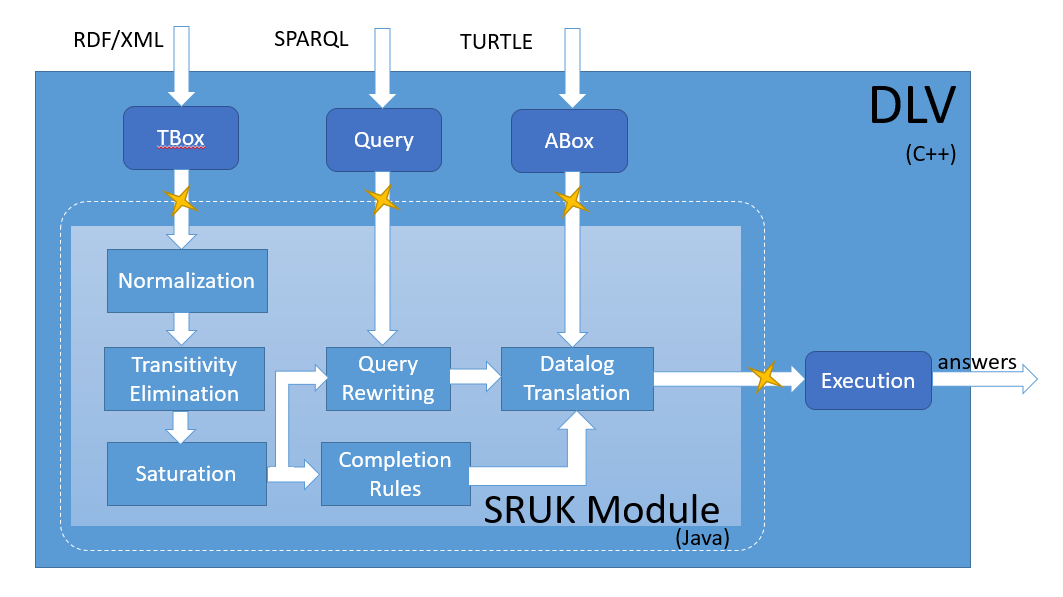
\includegraphics[width=1\linewidth]{Architecture}
% 	\caption{Architecture of the query rewriting module}
% 	\label{fig:architecture}
% \end{figure}

\subsection{Data Structures}

\subsubsection{TBox}
\begin{itemize}
\item Ontology classes: \textit{TBox},  \textit{ConceptInclusion},  \textit{RoleInclusion},  \textit{TransitivityAssertion}

\item Concept classes: \textit{Concept},  \textit{AtomicConcept},  \textit{NegatedConcept},  \textit{AndConcept},  \textit{OrConcept},  \textit{ExistentialConcept},  \textit{UniversalConcept},  \textit{MaxCardinalityConcept},  \textit{MinCardinalityConcept},  \textit{TopConcept},  \textit{BottomConcept}

\item Role classes: \textit{Role},  \textit{AtomicRole}
\end{itemize}



\subsubsection{ABox}
\textit{TBD}

\subsubsection{Query}
\begin{itemize}
	
	\item  \textit{UnionConjunctiveQuery},  \textit{ConjunctiveQuery},  \textit{Head},  \textit{Body},  \textit{Atom},  \textit{Term},  \textit{Variable},  \textit{Constant}
\end{itemize}


\subsubsection{Datalog Program}
\begin{itemize}
	
	\item  \textit{Program},  \textit{Rule},  \textit{Head},  \textit{Body},  \textit{Atom},  \textit{Term},  \textit{Variable},  \textit{Constant}
\end{itemize}


\subsection{Handling Datatypes}

For the first version we aim at supporting the following three datatypes.

\begin{itemize}
	\item \textit{xsd:integer}
	\item \textit{xsd:double}
	\item \textit{xsd:string}
\end{itemize}



%TBD: discuss how to properly translate axioms involving datatypes to Datalog rules.

\subsection{OWL Datatypes in DLV}
%Within our PoC, we agreed on supporting the following 3 standard OWL data types: xsd:string, xsd:integer, xsd:double. 
OWL data types will be supported by DLV via ad-hoc built-in functions. In particular, to state that the type of a variable X in a rule r should be either string, or integer or double the following atoms should be respectively used: $\&string(X;)$, $\&int(X;)$ and $\&double(X;)$. 

\

\textbf{Example 1}
The following DLV rule states that every individual X whose name is Y is a (valid) named individual only if Y is a string.
\[
namedIndividual(X) :- hasName(X,Y), \&string(Y;).
\]

%From OWL Datatypes to DLV
Our goal is to keep the in-memory knowledge base compliant with the datatype-constraints declared by the ontology. To accomplish this goal, we should rely on the following idea. Given a DatatypeProperty $R$ of range $T$, we must check that input ABox triples involving $R$ are compliant with the schema of $R$. Any triple violating the datatype-constraint over $R$ must be discarded at loading time and a warning message must be shown to point out the issue. Moreover, at rewriting time we must add a built-in atom $\&T(Y;)$ to the body of every rule where $R(X,Y)$ occurs in the head. The goal is to avoid the propagation of any tuple violating the datatype-constraint over $R$.

\

\textbf{Example 2}
Let $livesAt$ and address be two datatype properties such that address is a sub-property of $livesAt$. Moreover, the range of $livesAt$ is $xsd:string$ whereas the range of address is not specified. The aforementioned sub-property assertion is represented in DLV via the following rule:

\[
livesAt(X,Y) :- address(X,Y), \&string(Y;).
\]

Note that, an optimized version of the aforementioned approach would also consider the positions where $Y$ occurs in the body. In fact, if $Y$ occurs in the body only in positions of type T then the built-in atom $\&T(Y;)$ is not needed since we load in input only well-formed ABox triples.

\

\textbf{Example 3}
Let us consider the two datatype properties introduced in Example 2. Suppose that the range of address is $xsd:string$, as well as the range of $livesAt$. The sub-property assertion stating that address is a sub-property of $livesAt$ can be translated in DLV via the following rule:

\[
livesAt(X,Y) :- address(X,Y).
\]

In this case, the built-in atom $\&string(Y;)$ can be avoided because address may have only tuples with string values in the second position.

Other explicit restrictions involving OWL datatypes can be represented in DLV by using the syntax introduced above.

\subsection{IRI in DLV}

Ontologies and their elements are identified using Internationalized Resource Identifiers (IRIs). IRIs can be written as full IRIs by enclosing them in a pair of "$<$" and "$>$" characters. Alternatively, IRIs can be abbreviated as in SPARQL. 

To this end, one can declare a prefix name $pn$: — that is, a possibly empty string followed by the ":" character — by associating it with a prefix IRI $PI$; then, an IRI $I$ whose string representation consists of $PI$ followed by the remaining characters $rc$ can be abbreviated as $pn:rc$.

In general, IRIs are represented in DLV as full IRIs. Thus, any abbreviated form occurring in the OWL version of the input ontology must be resolved to a full IRIs. In particular, we need to distinguish between individuals and properties/classes. In fact, individual IRIs are represented in DLV as full IRIs enclosed between a pair of "" characters, whereas property/class names are represented as standard full IRIs.

\

\textbf{Example 1}

The following RDF triple

\[
\begin{array}{l}
<http://www.University0.edu> \\
<http://swat.cse.lehigh.edu/onto/univ-bench.owl\#name> \\
"University0"
\end{array}
\]
is represented as the following DLV fact:

\[
\begin{array}{l}
<http://swat.cse.lehigh.edu/onto/univ-bench.owl\#name>\\
(<http://www.University0.edu>", "University0").
\end{array}
\]



%%%%%%%%%%%%%%%%%%%%%%%%%%%%%%%%%%%%%%%%%%%%%%%%%%%%%%%%%%%%



\section{Design Magic Sets enhanced for Datalog-rewriting of OWL ontologies (Activity 2.3)}
Magic Sets are an optimization technique for addressing query answering in relational databases and logic-based systems. The technique is translational, from Datalog to Datalog in the context of this project, and therefore implementable as a module (almost) independent from other modules of DLV. The logic program in input is rewritten so that the subsequent bottom-up evaluation only materializes ground atoms that are relevant to answer the query in input. To this aim, new predicates are introduced in the rewritten program. Below is an example involving a recursive definition and asking for the descendants of mario:
\begin{verbatim}
  ancestor(X,Y) :- parent(X,Y).
  ancestor(X,Y) :- parent(X,Z), ancestor(Z,Y).
  ancestor(mario,X)?
\end{verbatim}

The Magic Sets rewriting starts with the query seed {\tt m\#ancestor\#bf(mario)}, modifies the rules defining the intentional predicate ancestor, and introduces magic rules for every occurrence of intentional predicates in the modified rules. The rewritten program is the following:
\begin{verbatim}
  m#ancestor#bf(mario).
  ancestor(X,Y) :- m#ancestor#bf(X), parent(X,Y).
  ancestor(X,Y) :- m#ancestor#bf(X),parent(X,Z),ancestor(Z,Y).
  m#ancestor#bf(Z) :- m#ancestor#bf(X), parent(X,Z).
\end{verbatim}

The rewritten program above is optimized for answering the specific query as its bottom-up evaluation only materializes descendants of mario, rather than the full ancestor relation.

There are cases in which several predicates for each predicate in the original program are introduced in the rewritten program. Below is an example, where all predicates are intentional, bindings are passed from left to right, and only rules defining the query predicate q are shown.
\begin{verbatim}
  q(X) :- r(a,X), s(X,Y), q(Y).
\end{verbatim}

The Magic Sets rewriting starts by introducing the magic seed {\tt m\#q\#f}. For each new predicate introduced by the rewriting, modified versions of the rules in input are added:
\begin{verbatim}
  q(X) :- m#q#f, r(a,X), s(X,Y), q(X).
\end{verbatim}
For each occurrence of an intentional predicate in a modified rule, a magic rule is added, possibly generating new predicates:
\begin{verbatim}
  m#r#bf(a) :- m#q#f.
  m#s#bf(X) :- m#q#f, r(a,X).
  m#q#b(Y) :- m#q#f, r(a,X), s(X,Y).
\end{verbatim}
The process is repeated, and the following rules are added:
\begin{verbatim}
  q(X) :- m#q#b(X), r(a,X), s(X,Y), q(X).
  m#r#bb(a,X) :- m#q#b(X).
  m#s#bf(X) :- m#q#b(X), r(a,X).
  m#q#b(Y) :- m#q#b(X), r(a,X), s(X,Y).
\end{verbatim}
At this point the rewriting reaches a fixpoint and terminates. Hence, the rewritten program contains the following rules (recall that the example is focused on the rules defining q, while the rules defining other intentional predicates have been omitted):
\begin{verbatim}
  m#q#f.
  q(X) :- m#q#f, r(a,X), s(X,Y), q(X).
  m#r#bf(a) :- m#q#f.
  m#s#bf(X) :- m#q#f, r(a,X).
  m#q#b(Y) :- m#q#f, r(a,X), s(X,Y).
  q(X) :- m#q#b(X), r(a,X), s(X,Y), q(X).
  m#r#bb(a,X) :- m#q#b(X).
  m#s#bf(X) :- m#q#b(X), r(a,X).
  m#q#b(Y) :- m#q#b(X), r(a,X), s(X,Y).
\end{verbatim}
Note that similar rules are introduced for predicates originating from the same source. Hence, a drawback of Magic Sets is the possible introduction of redundant rules and predicates.

Another possible source of inefficiency is the presence or the introduction of subsumed rules, that is, rules whose ground instances are included or less general than those associated with another rule in the program. Below is an example.
\begin{verbatim}
  q(X) :- p(X).
  q(X) :- p(X), t(X).
  q(a) :- p(a).
\end{verbatim}
We can observe that the first rules subsumes the other rules: ground instances of the second rule are less general than those of the first rule; the only ground instance of the third rule is among the the ground instances of the first rule.


\section{Implementation of Magic Sets enhanced for Datalog-rewriting of OWL ontologies (Activity 2.4)}

TODO


\chapter{Results}
[...]

Concerning Activity 2.3, our goal is to further optimize the Magic Sets technique by introducing postprocessing modules that identify redundant rules and predicates. Specifically, redundant rules are identified by a module that checks for subsumption, that is, rules whose ground instances are included or less general than those associated with another rule in the program are removed; the number of pairs of rules to be checked is significantly reduced by means of hashing techniques. Below is the result of the application of such a module to the example given in Section 2.3. 
\[
\begin{array}{l}
{\tt q(X) :- p(X).}\\
\mathtt{\stkout{q(X) :- p(X), t(X).}}\\
\mathtt{\stkout{ q(a) :- p(a).}}\\
\end{array}
\]


Intuitively, given two rules $r_1$, $r_2$, subsumption $r_1 \sqsubseteq r_2$ is checked by means of a backtracking procedure that searches for a substitution of the variables of r1 such that the head of $r_1$ matches the head of $r_2$, and the body of $r_1$ is a subset of the body of $r_2$. If such a substitution is found, rule  $r_2$ is removed. Checking all pairs is too expensive, and therefore each rule is associated with an hash value, currently of size 64 bits, computed as follows:
\begin{itemize}
\item <OR of IDs of head predicates>, 8 bits;
\item <OR of IDs of head constants>, 8 bits;
\item <OR of IDs of predicates in positive body>, 16 bits;
\item <OR of IDs of constants in positive body>, 16 bits;
\item <OR of IDs of predicates in negative body>, 8 bits;
\item <OR of IDs of constants in negative body>, 8 bits.
\end{itemize}
Subsumption $r_1 \sqsubseteq r_2$ is checked only if the following bit-a-bit equation is satisfied:
$$hash(r_1) \ \& \ hash(r_2) == hash(r_1)$$
In the example above, the third rule cannot subsume the other rules because of the constant a, and the second rule cannot subsume the other rules because of the predicate t; depending on the IDs associated with predicates and constants, the hashing technique can detect this fact and avoid the backtracking searches.

The module that identifies redundant predicates, instead, takes into account the different bindings associated with predicates originating from the same source, and eliminates the rules associated with the more bounded predicates. In the example given in Section 2.3, predicate {\tt m\#q\#b} is more bounded than predicate {\tt m\#q\#f}, and therefore the rules associated with {\tt m\#q\#b} are removed. Similarly, rules associated with {\tt m\#r\#bb} and {\tt m\#s\#bf} are removed. Hence, the rewritten program, focused on the rules defining q, is the following:
\[
\begin{array}{l}
	{\tt m\#q\#f.}\\
	{\tt q(X) :- m\#q\#f, r(a,X), s(X,Y), q(X).}\\
	{\tt m\#r\#bf(a) :- m\#q\#f.}\\
	{\tt m\#s\#bf(X) :- m\#q\#f, r(a,X).}\\
	\mathtt{\stkout{m\#q\#b(Y) :- m\#q\#f, r(a,X), s(X,Y).}}\\
	\mathtt{\stkout{q(X) :- m\#q\#b(X), r(a,X), s(X,Y), q(X).}}\\
	\mathtt{\stkout{m\#r\#bb(a,X) :- m\#q\#b(X).}}\\
	\mathtt{\stkout{m\#s\#bf(X) :- m\#q\#b(X), r(a,X).}}\\
	\mathtt{\stkout{m\#q\#b(Y) :- m\#q\#b(X), r(a,X), s(X,Y).}}\\
\end{array}
\]
[...]




\chapter{Open research issues}
\chapter{Bibliography}
\chapter{Appendix}


%%%%%%%%%%%%%%%%%%%%%%%%%%%%%%%%%%%%%%%%%%%%%%%%%%%%%%%%%%%%%%%%%%%%%%%%%%%%%%%%%%%%%%%%%%%%%%%%%%%%%%%%%%%%%%%%%%%%%%%%
%%%%%%%%%%%%%%%%%%%%%%%%%%%%%%%%%%%%%%%%%%%%%%%%%%%%%%%%%%%%%%%%%%%%%%%%%%%%%%%%%%%%%%%%%%%%%%%%%%%%%%%%%%%%%%%%%%%%%%%%
%%%%%%%%%%%%%%%%%%%%%%%%%%%%%%%%%%%%%%%%%%%%%%%%%%%%%%%%%%%%%%%%%%%%%%%%%%%%%%%%%%%%%%%%%%%%%%%%%%%%%%%%%%%%%%%%%%%%%%%%
\setcounter{chapter}{0}

\part*{Work Package 3:\\Enhancing the SPARQL Query Evaluation/Execution Procedure}
\addcontentsline{toc}{part}{WP3: Enhancing the SPARQL Query Evaluation/Execution}

\chapter{Scenario and problem description}

DLV has been designed as an in-memory system allowing only one-shot executions. In particular, when it is run on a specific input the system starts, loads input data, processes the requested query and stops as soon as the computation is completed. However, when multiple queries are evaluated over the same input data, the aforementioned behaviour could be rather expensive since the system needs to reload input data at each run and for each query. Within WP3, we aim at extending the system by providing a server-like behaviour that allows to keep the main process alive also after the computation is performed. In this way, DLV will be able to answer multiple queries over the same input knowledge base without loading input data more than once. More in detail, we plan to further equip the DLV server version with the following useful functionalities:
\begin{itemize}
\item Load ontology
\item Load data (in form of logic fact or RDF triple)
\item Add data (in form of logic fact or RDF triple)
\item Remove data (in form of logic fact or RDF triple)
\item Run query
\item Reset ontology
\item Reset data
\item Compute statistics for query optimizations
\end{itemize}

A further goal of WP3 is to study and develop suitable optimization techniques intended to speed-up the execution of query-programs on given query-patterns (e.g., advanced indexing and ordering techniques). Finally, the last goal of this work package is to reduce the memory consumption of DLV in order to permit the handling of large scale knowledge bases characterized by ABoxes featuring billions of triples.
BLA BLA BLA… 



\section{Team}
WP3 has been jointly developed by DLVSystem and DeMaCS@UNICAL. In particular, what follows is the list of the involved researchers: Francesco Calimeri (Professor), Roberta Costabile (PhDStudent), Alessio Fiorentino (PhDStudent), Davide Fuscà (PostDoc), Simona Perri (Professor), Kristian Reale (PostDoc), Francesco Ricca (Professor), Jessica Zangari (PostDoc).

\section{Activity title}
TODO
\section{Activity title}
TODO
\section{Activity title}


\chapter{Results}
\chapter{Open research issues}
\chapter{Bibliography}
\chapter{Appendix}

%%%%%%%%%%%%%%%%%%%%%%%%%%%%%%%%%%%%%%%%%%%%%%%%%%%%%%%%%%%%%%%%%%%%%%%%%%%%%%%%%%%%%%%%%%%%%%%%%%%%%%%%%%%%%%%%%%%%%%%%
%%%%%%%%%%%%%%%%%%%%%%%%%%%%%%%%%%%%%%%%%%%%%%%%%%%%%%%%%%%%%%%%%%%%%%%%%%%%%%%%%%%%%%%%%%%%%%%%%%%%%%%%%%%%%%%%%%%%%%%%
%%%%%%%%%%%%%%%%%%%%%%%%%%%%%%%%%%%%%%%%%%%%%%%%%%%%%%%%%%%%%%%%%%%%%%%%%%%%%%%%%%%%%%%%%%%%%%%%%%%%%%%%%%%%%%%%%%%%%%%%
\setcounter{chapter}{0}

\part*{Work Package 4:\\Test Case Design}
\addcontentsline{toc}{part}{WP4: Test Case Design}

\chapter{Scenario and problem description}

Within activity A4.1, we aim at building a benchmark domain for evaluating powerful ontology reasoners relying on a non-materialization approach over a large dataset (more than 1 billion triples), where the latter is constantly subject to evolution (addition or deletion of triples from the ABox). The goal of this activity is to appropriately select and extend, if possible, an existing OWL benchmark for evaluating ontology reasoners against a large knowledge base with (near-)real time data. In particular, we must consider only benchmarks that enjoy the following main requirements:
\begin{enumerate}
\item the data generator is able to generate more than 1 billion triples;
\item the ontology expressiveness is as close as possible to OWL 2 DL;
\item the benchmark evaluates the tested systems over a dynamic dataset. 
\end{enumerate}
In order to simulate a dynamic evolution of the knowledge base, the tested systems will be required to load an initial large dataset (close to 1 billion triples) and answer a fixed set of queries. Next, at a frequency $f=\frac{1}{\Delta T}$ where $\Delta T$ is a given time period,  $x\%$ of the initial number of triples will be either deleted or generated and added to the ABox. After the systems are notified of the underlying knowledge base changes, they will have to answer again the fixed set of queries. Hence, the frequency $f$ and the rate $x\%$ (expressed as percentage of the initial number of triples) of the instance deletions/additions should be a tuneable parameter of our benchmark. 

Currently, the research effort provide a number of well-established benchmarks, including LUBM, UOBM, BSBM and SPB. LUBM has been designed for comparing performance, soundness and completeness of OWL reasoning engines, against a static knowledge base. UOBM extends LUBM by adding axioms that make use of all OWL Lite and OWL DL constructs. BSBM aims at comparing the performances of systems that expose SPARQL endpoints, and can simulate different real-world scenarios. Similarly, the Semantic Publishing Benchmark (SPB) can simulate a real-world scenario where a number of aggregation agents provide the heavy query workload, while at the same time a steady stream of editorial agents execute a number of update operations.

According to the requirements introduced above, none of the aforementioned benchmarks can be used without being extended for our purpose. Indeed, UOBM features an ontology going beyond Horn-SHIQ and it does not provide any official (dynamic) data generator. BSBM includes some queries requiring either aggregates or string functions and it does not provide any way to simulate data evolution. SPB does provide a reliable data generator and it can simulate a dynamic environment but its ontology is too easy to handle since its expressiveness falls into OWL 2 RL. Finally, LUBM does not simulate a dynamic environment. 

However, this latter benchmark seems to be the most suitable choice since it could be easily extended for our purpose. Indeed, it provides an expressive ontology (falling into Horn-SHIQ and going beyond OWL 2 RL), a reliable data generator (which can be exploited to generate huge instances and to produce axioms to be added during the ABox evolution) and a set of 14 SPARQL queries.


Hence, the main goal of activity A4.1 is to equip LUBM with a test driver that allows simulating a dynamic evolution of the initial dataset, by adding/deleting $x\%$  of the initial number of triples at a frequency $f=\frac{1}{\Delta T}$ (notice that both $\Delta T$ and $x$ should be tuneable parameters of our test driver). Moreover, we aim at devising more complex queries to fully exploit expressiveness of the LUBM ontology since 9 out of the original 14 queries can be now handled by any OWL 2 RL reasoner.
BLA BLA BLA… 


\section{Team}
WP1 has been jointly developed by DLVSystem and SRUK. In particular, what follows is the list of the involved researchers: Pierfrancesco Veltri (PostDoc), Maud Lemercier (Software Engineer).

\section{Activity title (A4.1)}
TODO
\section{Activity title (A4.2)}
TODO
\section{Activity title (A4.3)}


\chapter{Results}
\chapter{Open research issues}
\chapter{Bibliography}
\chapter{Appendix}


\end{document}
